% ┌────────────────────────────────────────────────────────────────────────────┐
% │ ALU PAPER                                                                  │
% │   Evolution shapes the RNA metabolism of Alu retrotransposons              │
% └────────────────────────────────────────────────────────────────────────────┘

\chapter{Evolution Shapes the Alu RNA Metabolism}
\sectionmark{Evolution Shapes the Alu RNA Metabolism}

In this explorative study, we looked into the lifecycle of Alu elements,
retrotransposons in the human genome that copy themselves into new genomic
positions. We wanted to answer four questions concerning the transcription
and degradation of Alu RNAs and the sequence features that influence these
processes.

Alu elements, classified as short interspersed nuclear elements (SINEs), are
around \num{300}~bp long mobile DNA sequences found in the human genome and
other species \citep{Quentin1992,Lander2001a,JO2007,Deininger2011}. They are
RNA retrotransposons, meaning that they are capable of copying themselves into
new positions in the genome. Due to this multiplication, Alu elements make up
\SI{11}{\percent} of the human genome by length, with more than \num{1}
million currently annotated loci \citep{Lander2001a}.

The retrotransposition process of Alu elements shown in \cref{fig:alulife},
however, is error-prone and thus facilitates an Alu-specific sequence
evolution, giving rise to distinct Alu families from the old AluJ family over
AluS to the young AluY \citep{MR1991,PL1992,Batzer1996}. In general, Alu
elements are composed of a left arm and a right arm separated by a variable A-
rich region \citep{Evgenev2007}. The left arm contains an RNA Polymerase III
(Pol-III) promoter\label{sen:alupromo}, and the right arm holds the UGU(NR)
motif required for binding to the ribosome (see \cref{fig:alulife})
\citep{ Paolella1983,Dagan2004,A2012}. If Alu elements serve a function is,
so far, unknown. They can be harmful if a new insertion disrupts a gene or
other genomic region \citep{PL1999}. They have also been linked to changes in
transcriptional activity in general and under heat shock conditions in
particular \citep{Mariner2008,LL2017,Zhang2019}.

We wanted to address four questions regarding Alu elements, their
transcription, and their sequence features:

\begin{figure}[b!]
\centering
 \makebox[\textwidth][r]{
   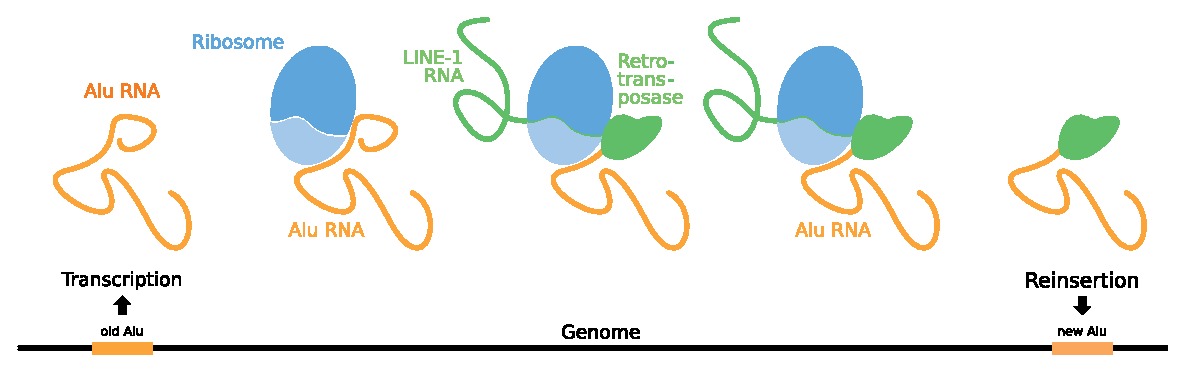
\includegraphics[width=\textwidth+\marginparwidth+\marginparsep]{
     04_GraphicFiles/02_alu_life.eps}}
\caption{Modification of figure 1a from \citet{Baar2022}, showing a schematic
  representation of Alu retrotransposition (left to right): the Alu element
  is transcribed -- the Alu RNA attaches itself to the exit tunnel of the
  ribosome through its SRP sequence homolog -- a LINE-1 RNA arrives at the
  ribosome and its retrotransposase is translated -- the Alu RNA hijacks the
  LINE-1 retrotransposase -- the LINE-1 retrotransposase reinserts the Alu
  element into a new genomic position.}
\label{fig:alulife}
\end{figure}

\begin{enumerate}[labelindent=0pt]
  \item Are Alu RNAs stable or unstable?\smallskip\newline
  Previous studies suggested that Alu RNAs should be less stable in the cell
  than regular mRNAs, meaning that they are degraded quickly \citep{An2004}.
  However, these results were obtained using only computational methods
  extrapolating from Alu sequence features and were not backed up by
  experimental data.\newline
  We could show that the distribution of Alu RNA half-lives predicted by our
  experimental approach is very similar to that of mRNAs, suggesting that Alu
  transcripts are more stable than previously thought.

  \item Are Alu elements transcribed primarily by Pol-III or by RNA
  Polymerase II (Pol-II), as well?\smallskip\newline
  While Alu elements do contain a Pol-III promoter sequence (see
  \cpageref{sen:alupromo}), it is surmised that Alu elements are not only
  transcribed by Pol-III but also, to a certain extent, by Pol-II
  \citep{Conti2015a,Zhang2019}. The experimental evidence for this is mostly
  indirect \citep{ Zhang2019,Panning1993,JAGADEESWARAN1981}. We have therefore
  conducted a Pol-II inhibition experiment and could show that Alu expression
  does indeed decrease under Pol-II inhibition, suggesting strongly that Alu
  transcripts arise, at least in part, directly from Pol-II activity.\newline
  This finding carries implications for differential expression analyses of
  the past. Often, Alu elements were used as a control group if Pol-II
  inhibition was performed, assuming wrongly that Alu transcription should be
  completely dependent on Pol-III \citep{Cordaux2009}.
  
  \item Is Alu transcription a side product of gene
  transcription?\smallskip\newline
  If a fraction of Alu transcription depends on Pol-II activity, a possible
  explanation could be that Alu elements are transcribed alongside regular
  genes \citep{Conti2015a,Zhang2019}. The results of our analyses weaken this
  hypothesis. While we cannot rule out that a fraction of Alu elements might
  be transcribed alongside genes, it is unlikely that this process contributes
  substantially to Alu expression.
  
  \item Is Alu expression influenced by sequence features?\smallskip\newline
  Previous studies unsuccessfully employed regular \textit{de novo} motif
  search to detect Alu sequence features that influence their expression
  \citep{Zhang2019}. We used two less common methods (see
  \nameref{subsubsec:aluanalysis}) and could uncover several influential
  positions and motifs that appear linked to changes in Alu expression.
  Additionally, some of the motifs match transcription factor binding profiles
  and may thus present promising targets for future investigations.
\end{enumerate}

\subsubsection{Methodology}\label{subsubsec:alumethod}
\addcontentsline{toc}{subsection}{Methodology}
This study made use of bulk, whole-genome RNAseq data, partially generated
specifically for our investigation and partially repurposed from our earlier
publication \citet{Schwalb2016}. The RNA was extracted from K562 cells, an
immortalised human suspension cell line of erythroleukemia cells
\citep{Andersson1979}. The sequencing data is noteworthy regarding two of its
characteristics:

Firstly, we used dynamic transcriptome analysis (DTA), specifically the 4sUseq
and the TTseq methods \citep{Schwalb2012,Gressel2019}. DTA chemically labels
newly created transcripts, making them distinguishable from old RNAs still
present from before the labelling pulse. This allowed us to calculate the
ratio between old and new transcripts and thereby estimate these transcripts'
half-life.

Secondly, we performed a Pol-II inhibition experiment using \textalpha-%
amanitin, a toxic substance from the \textit{Amanita phalloides} fungus that
blocks Pol-II activity \citep{Lindell1970,Kedinger1970,Stirpe1967,Jacob1970}.
We treated K562 cells with \textalpha-amanitin and compared their RNAseq data
with untreated samples. We could thus observe the effect of Pol-II inhibition
on different transcript classes, including Alu elements, \textit{bona fide}
Pol-II genes, and tRNAs, which are transcribed by the uninhibited Pol-III.

\subsubsection{Analysis}\label{subsubsec:aluanalysis}
\addcontentsline{toc}{subsection}{Analysis}

% ┌────────────────────────────────────────────────────────────────────────────┐
% │ 1. Are Alu RNAs stable or unstable?                                        │
% │    Half-Life Estimation                                                    │
% └────────────────────────────────────────────────────────────────────────────┘

Concerning\marginnote{Half-Life Estimation}\label{mar:alumle} the question,
if Alu RNAs are stable or unstable, we relied on the DTA data (see
\nameref{subsubsec:alumethod}), giving us two read counts for each Alu
element or gene, one from the labelled fraction and one from the total
fraction. With time, new labelled transcripts are created and old unlabelled
transcripts decay, meaning that the ratio of labelled RNAs increases until all
transcripts are labelled. Assuming exponential decay and steady-state
conditions, this ratio $r_{a}$ gives us the decay rate $\delta{}_{a}$ for any
Alu element or gene $a$ by
\begin{align*}
       r_{a} &= \nicefrac{l_{a}}{t_{a}}=1-\exp(-\delta_{a}\Delta t)
\\ \ln r_{a} &= \ln\left(1-\exp(-\delta_{a}\Delta t)\right)
\end{align*}
where $l_{a}$ and $t_{a}$ are the numbers of labelled or total RNA molecules
and $\Delta{}t$ is the labelling pulse’s duration, meaning the time that
passed after the labelling agent was added and before the RNA sequencing was
performed. From the decay rate $\delta{}_{a}$ the half-life
$t_{\nicefrac{1}{2}}$ is given by
\begin{align*}
t_{\nicefrac{1}{2}}=\frac{\ln\left(2\right)}{\delta}
\end{align*}
To estimate the ratio between labelled and total RNA molecules from the
measured reads, we used maximum likelihood estimation (MLE) \citep{Rossi2018}
(see also \nameref{sec:methoverview}). We made several assumptions to simplify
the estimation, owing to the general paucity of Alu read counts caused by
their low expression. We assume steady-state conditions, use a Poisson
distribution to model read counts instead of a zero-inflated negative binomial
distribution, and neglect non-constant labelling efficiencies for short
labelling periods. This means that our estimation can only serve as an
assessment to compare the relative half-life distributions of Alu elements and
genes. Its predictions do not represent explicit half-life values. Still, the
very similar distribution of Alu and gene half-lives suggests that the
stability of Alu transcripts is greater than would be expected from sequence
features alone.
\bigbreak

\begin{figure}[b!]
\centering
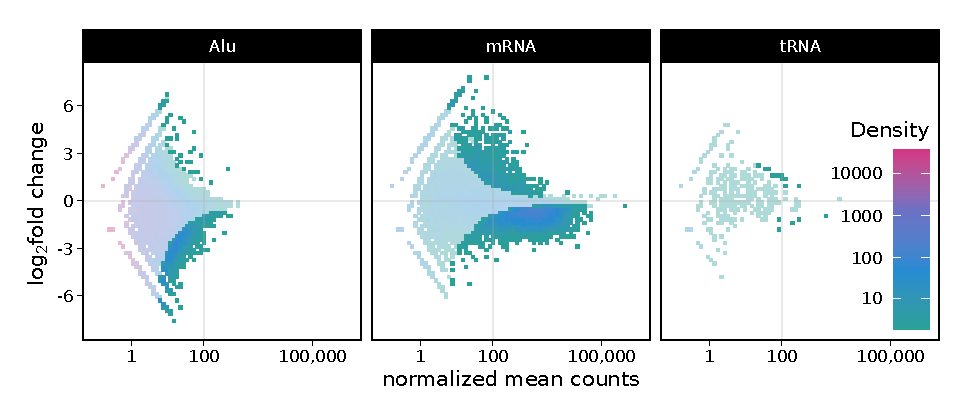
\includegraphics[width=\textwidth]{04_GraphicFiles/02_alu_deseq2.eps}
\caption{Modification of figure 3e from \citet{Baar2022}. 2D density heatmap
  showing the DESeq2 differential expression of Alu elements, mRNAs, and tRNAs
  under \textalpha-amanitin Pol-II inhibition. Semi-transparent areas do not
  pass the significance threshold. Loci with a normalised mean expression
  below 0.1 are excluded, with affects \SI{51}{\percent} of all annotated
  Alu loci and practically no mRNAs or tRNAs.}
\label{fig:aludeseq2}
\end{figure}

\noindent The \textalpha-amanitin\marginnote{Differential Expression Analysis}
\label{mar:aludeseq2} Pol-II inhibition experiment was the key to
investigating the origin of Alu transcripts. To analyse the RNAseq
measurements, we used the DESeq2 package for R \citep{Love2014}. The standard
assumption of DESeq2's internal normalisation strategy is that there are no
substantial, systematic global expression changes between samples. Due to the
inhibition of Pol-II, we have to assume that this does not hold. We,
therefore, used mitochondrial transcripts (mtRNAs) for normalisation, which
are unaffected by the \textalpha-amanitin treatment. This is because the
mitochondrial polymerase that transcribes mtRNAs is not inhibited by
\textalpha-amanitin \citep{Menon1971,Reid2830,Saccone1971}. The resulting
differential expression estimates of Alu elements, mRNAs, and tRNAs, which we
used as a negative control as they are transcribed by Pol-III, which is also
unaffected by \textalpha-amanitin, are shown in \cref{fig:aludeseq2}
\citep{ White1997}. As expected, tRNAs remain largely unaffected by the
\textalpha-amanitin treatment, while mRNAs exhibit downregulation. Notably,
Alu RNAs also appear downregulated under Pol-II inhibition, suggesting
strongly that Alu elements are, at least to a certain extent, transcribed by
Pol-II.
\bigbreak

\noindent To address\marginnote{Correlation Analysis}\label{mar:alucor} the
follow-up question if the apparent expression of Alu elements by Pol-II may
result from Alu RNAs being side products of gene transcription, we argued as
follows \citep{Conti2015a,Zhang2019}: If Alu elements were transcribed
alongside genes, those inside or close to genes should show higher expression
compared to Alu elements that are far away from genes. The expression of a
gene should also correlate with the expression of Alu elements inside or close
to it. Finally, Alu elements should show a bias towards lying in sense
direction with regard to their associated gene.

While we did detect a significantly higher expression of Alu elements that lie
inside or close to genes, this effect can result easily from increased genome
accessibility in areas of active gene transcription \citep{Guo2016}. This also
biases the correlation analysis. Therefore, we examined the difference in
correlation strength between Alu element and gene transcription if split by
sense and antisense Alu direction. As we detected no difference in correlation
strength and also found that Alu elements show no preference for inserting
themselves in sense direction into genes, we conclude that it is unlikely that
Alu transcription is a side product of gene transcription. While our results
do not rule out that some Alu transcripts are created alongside genes, this
does not appear to be a major source for Alu RNAs.
\bigbreak

\noindent To search\marginnote{Generalised\\ Linear Model}\label{mar:aluglm}
for sequence features that influence Alu expression, we pursued two different
approaches. Firstly, to analyse Alu elements on a per-base level, we used a
generalised linear model created with the glmnet package for R
\citep{Nelder1972, Friedman2010} (see also \nameref{sec:methoverview}). We
assumed a Poisson family distribution response type and used an elastic mixing
parameter \textalpha{} of \num{1} (full Lasso penalty, no ridge regression
penalty), no fitted intercept parameter, and \num{1000}$\times$ cross-%
validation. To create the input matrices, we aligned all Alu sequences against
the Alu consensus sequence and encoded base exchanges, deletions, and
insertions for each position as a binary matrix. For these three types of
point mutation, we trained GLMs with the Alu read counts as a response
variable. Finally, we used the Euclidean norm of the three obtained effect
sizes for each position in the Alu consensus sequence to judge their
respective importance, uncovering several influential positions.
\bigbreak

\noindent Secondly,\marginnote{De Bruijn Graph}\label{mar:alugraph} to detect
larger sequence features, we created a De Bruijn graph of all Alu sequences
using bifrost v1.0.5 \citep{Holley2020} (see also \nameref{sec:methoverview}).
As the graph was almost complete with an in-degree per node of \num{>7.99}, we
focused on the constituent k-mers and disregarded the graph structure in
downstream analyses. We filtered the k-mers using two criteria. The expression
of Alu elements possessing the k-mer needed to be significantly different from
those not possessing it. Also, we took each k-mers's suffix and prefix into
account.

Assuming a k-mer with the structure $\text{X\,J\,Y}$, with
$\text{X},\text{Y}\in\{A,C,T,G\}$ and $\text{J}$ a fixed 2-mer, to assure that
$\text{X\,J\,Y}$ is causal for observed changes in Alu transcription, we test
the group of Alu elements containing $\text{X\,J\,Y}$ against the group
containing the k-mer's prefix $\text{X\,J}$ or its suffix $\text{J\,Y}$, but
not the full k-mer. Thus we can be confident that the observed effect is
caused by the complete k-mer and not just its partial sequence.

\noindent With this method. we uncovered several statistically significant and
biologically relevant sequence motifs which previous attempts using regular
\textit{de novo} motif search did not \citep{Zhang2019}.
\bigbreak

\noindent In summary, we found that Alu transcripts appear to be as stable as
mRNAs, more stable than previously thought. In addition, we found evidence for
Alu elements originating in independent Pol-II transcription, not originating
as side products of gene transcription. Finally, we also identified a list of
sequence features that influence Alu expression and might therefore be
promising targets for future investigations.

\vfill
\noindent My contribution to this publication was the complete bioinformatic
and statistical analysis.\nopagebreak
\medskip
\begin{tcolorbox}[
  boxrule=0pt, leftrule=1pt, colframe=s-blue, colback=white, sharp corners=all]%
  \raggedright
  Baar, T., Dümcke, S., Gressel, S., Schwalb, B.,
  Dilthey, A., Cramer, P., Tresch, A. (2022).
  
  \smallskip
  \href{https://doi.org/10.1093/g3journal/jkac054}
    {RNA transcription and degradation of Alu retrotransposons depends on
    sequence features and evolutionary history}

  \smallskip
  \textit{G3: Genes}\thinspace{}|\thinspace{}\textit{Genomes}%
    \thinspace{}|\thinspace{}\textit{Genetics, ???}
\end{tcolorbox}